\begin{figure}
\begin{fullwidth}
\centering
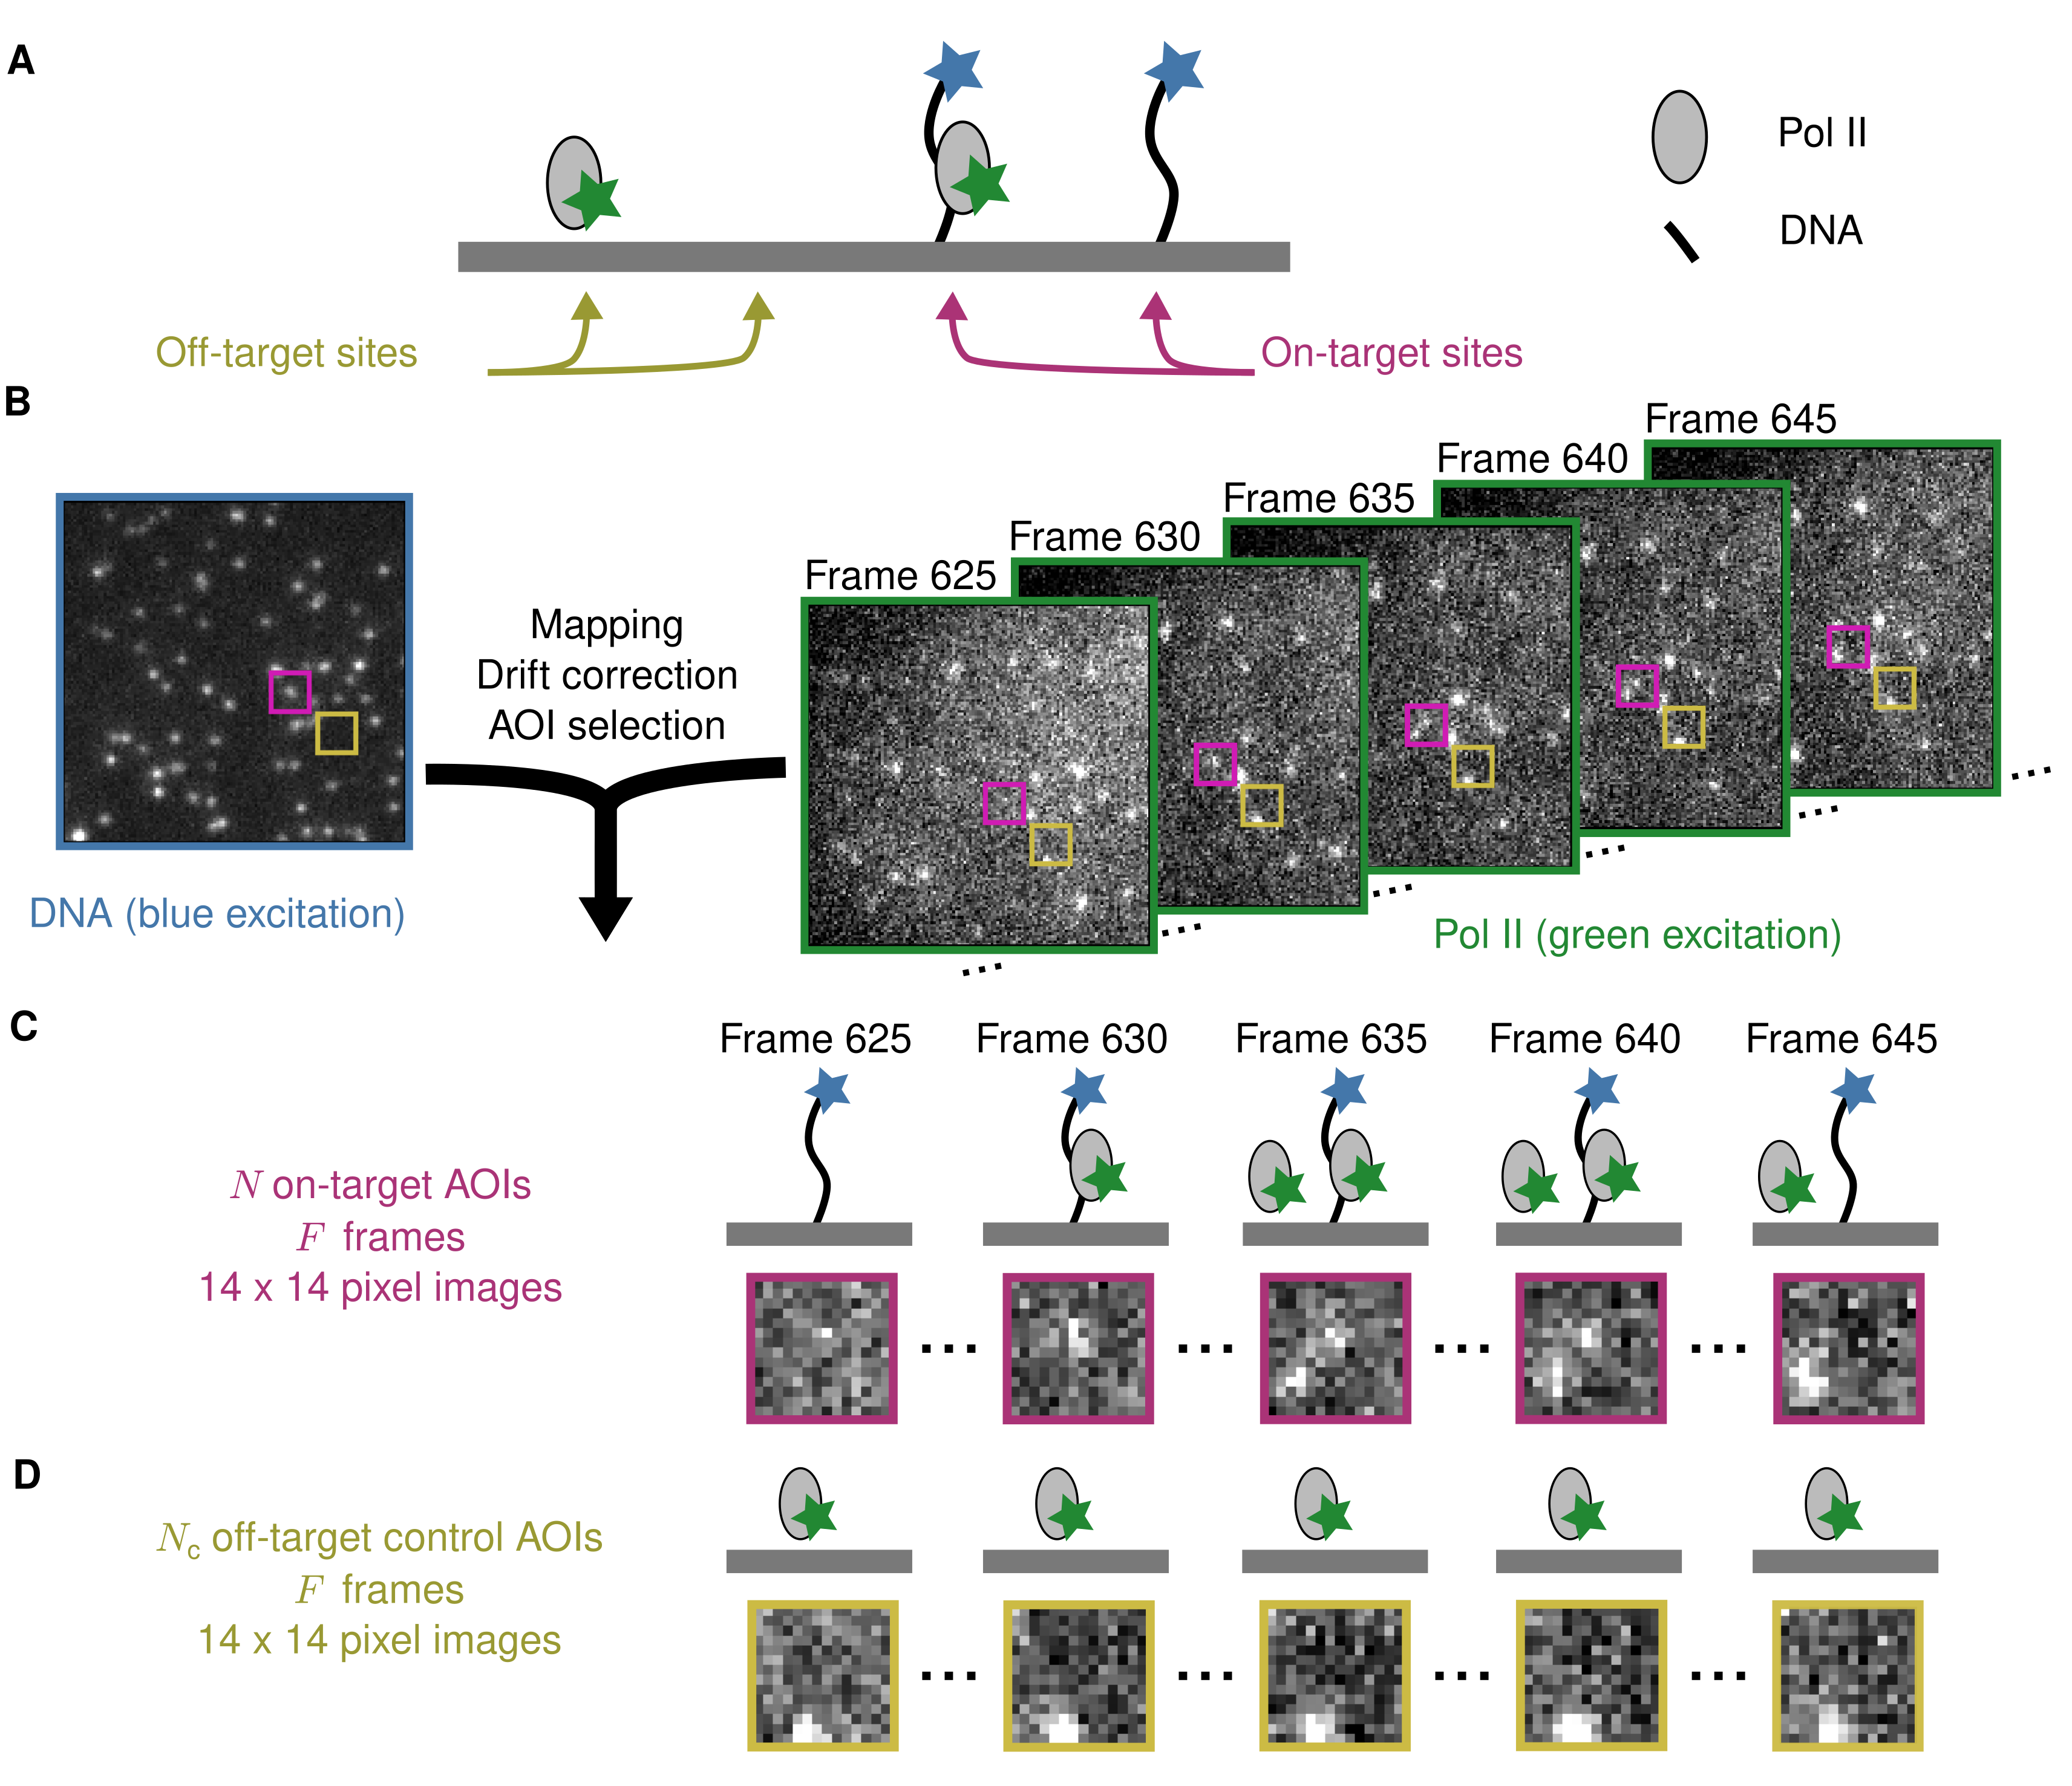
\includegraphics[width=145mm]{figures/cosmos_experiment/cosmos_experiment.png}
\caption{\textbf{Example CoSMoS experiment.} Data set A in \TABLE{datasets}. (\textbf{A}) Experiment schematic. DNA target molecules labeled with a blue-excited fluorescent dye (blue star) are tethered to the microscope slide surface. RNA polymerase II (Pol II) binder molecules labeled with a green-excited dye (green star) are present in solution. (\textbf{B}) Data collection and preprocessing. After collecting a single image with blue excitation to identify the location of the DNA molecules, a time sequence of Pol II images were collected with green excitation.  Preprocessing of the images includes mapping of the corresponding points in target and binder channels, drift correction, and identification of two sets of areas of interest (AOIs).  One set corresponds to locations of target molecules (e.g., purple square); the other corresponds to locations where no target is present (e.g., yellow square). (\textbf{C}) On-target data. Data are time sequences of 14 $\times$ 14 pixel AOI images centered at each target molecule. Frames show presence of on-target (e.g., frame 630) and off-target (e.g., frame 645) Pol II molecules. (\textbf{D}) Off-target control data. Control data consists of images collected from randomly selected sites at which no target molecule is present. }
\label{fig:cosmos_experiment}
\end{fullwidth}
\end{figure}